\documentclass[11pt,a4paper]{article}
\usepackage[utf8]{inputenc}
\usepackage[T1]{fontenc}
\usepackage[brazilian]{babel}
\usepackage[margin=2.2cm]{geometry}
\usepackage{graphicx}
\usepackage{booktabs}
\usepackage{xcolor}
\usepackage{listings}
\usepackage{hyperref}
\usepackage{float}
\usepackage{tikz}
\usetikzlibrary{positioning}

\hypersetup{
    colorlinks=true,
    linkcolor=blue!60!black,
    urlcolor=blue!60!black
}

\lstset{
    basicstyle=\ttfamily\footnotesize,
    breaklines=true,
    frame=single,
    backgroundcolor=\color{gray!8},
    rulecolor=\color{gray!40},
    columns=flexible,
    keepspaces=true
}

\title{
    \textbf{Pontifícia Universidade Católica do Rio Grande do Sul}\\
    \large Escola Politécnica --- Fundamentos de Redes de Computadores\\[0.6em]
    \Large \textbf{Relatório Técnico: Protocolo de Roteamento Link State (OSPF-like)}
}
\author{Diego Mello}
\date{18 de novembro de 2026}

\begin{document}
\maketitle
\tableofcontents
\newpage

\section{Arquitetura da Solução}

A aplicação foi desenvolvida em \textbf{Go} (\texttt{go1.21+}) utilizando comunicação via sockets UDP (\texttt{net.UDPConn}), seguindo integralmente a especificação do protocolo Link State proposto. A arquitetura foi dividida em pacotes bem definidos:

\begin{itemize}
    \item \texttt{main.go}: ponto de entrada da aplicação, responsável pelo parsing de argumentos de linha de comando (\texttt{-ip}, \texttt{-port}, \texttt{-local}, \texttt{-dir}, \texttt{-peers}, \texttt{-bind}) e encerramento gracioso via sinais do sistema operacional.
    \item \texttt{internal/protocol/messages.go}: codificação, decodificação e validação estrita dos datagramas \texttt{HELLO} (\texttt{@}), \texttt{LSA} (\texttt{\#}) e \texttt{DATA} (\texttt{!}), garantindo codificação UTF-8, identificadores IPv4 canônicos, tamanho máximo de \texttt{1200} bytes e ausência de quebra de linha ao final.
    \item \texttt{internal/routing/dijkstra.go}: construção do grafo direcionado a partir da LSDB, implementação própria do algoritmo de Dijkstra (sem bibliotecas externas de caminhos mínimos) e detecção de alterações na tabela de roteamento (\texttt{DiffRoutes}).
    \item \texttt{internal/router/config.go}: leitura e persistência de \texttt{roteadores.txt} (vizinhos configurados e custos), gravação síncrona de \texttt{seq.txt} antes de cada novo LSA e suporte a mapeamento de portas locais (\texttt{peers.txt}).
    \item \texttt{internal/router/router.go}: núcleo concorrente do roteador (goroutines \texttt{receiveLoop} e \texttt{timerLoop}), gerenciando vizinhos, LSDB, \emph{flooding}, expiração de anúncios, timeouts e encaminhamento de pacotes \texttt{DATA}.
    \item \texttt{internal/router/cli.go}: interface interativa via terminal para consulta da LSDB, tabela de roteamento e vizinhos, além de manipulação dinâmica da topologia sem reiniciar o processo.
\end{itemize}

\subsection{Modos de Execução}
\begin{itemize}
    \item \textbf{Modo Especificação (padrão):} escuta em \texttt{0.0.0.0:6000} e utiliza os endereços IPv4 reais listados em \texttt{roteadores.txt}, permitindo interoperabilidade direta entre diferentes computadores e implementações de outros grupos na porta UDP \texttt{6000}.
    \item \textbf{Modo Local Loopback (\texttt{-local}):} escuta em \texttt{127.0.0.1:<porta>} (ex.: \texttt{6000} a \texttt{6003}) preservando os identificadores IPv4 lógicos (\texttt{10.0.0.1} a \texttt{10.0.0.4}) dentro dos datagramas, viabilizando testes completos em uma única máquina sem conflito de porta.
\end{itemize}

\section{Estruturas de Dados e Temporizadores}

\subsection{Estruturas Principais}
\begin{enumerate}
    \item \textbf{Tabela de Vizinhos (\texttt{map[string]*NeighborState}):} armazena para cada vizinho configurado o endereço \texttt{IP}, o custo positivo do enlace (\texttt{Cost}), a flag de desativação lógica (\texttt{Disabled}), o estado da adjacência (\texttt{Active}) e o instante do último \texttt{HELLO} válido (\texttt{LastHello}).
    \item \textbf{LSDB (\texttt{map[string]routing.LSARecord}) e Controle de Sequência (\texttt{maxSeq}):} cada entrada guarda \texttt{OriginIP}, \texttt{Sequence}, \texttt{Links} (\texttt{map[string]int}) e \texttt{ReceivedAt}. O mapa auxiliar \texttt{maxSeq map[string]int} preserva, durante toda a execução, o maior número de sequência já aceito de cada origem mesmo após expiração na LSDB, bloqueando anúncios antigos ou duplicados.
    \item \textbf{Tabela de Roteamento (\texttt{map[string]routing.Route}):} mapeia cada destino (exceto o próprio IP) para \texttt{TotalCost} e \texttt{NextHop} (sempre um vizinho ativo).
    \item \textbf{Persistência de Sequência (\texttt{seq.txt}):} o número de sequência local inicia em 1, é incrementado a cada novo LSA (inclusive renovações periódicas) e gravado em \texttt{seq.txt} \emph{antes} do envio.
\end{enumerate}

\subsection{Temporizadores}
No loop \texttt{timerLoop} (\texttt{internal/router/router.go}), quatro temporizadores governam o protocolo:
\begin{table}[H]
\centering
\begin{tabular}{@{}lll@{}}
\toprule
\textbf{Temporizador} & \textbf{Intervalo} & \textbf{Função} \\
\midrule
\texttt{HelloInterval}   & 5 s  & Envio periódico de \texttt{HELLO} aos vizinhos configurados e ativos/habilitados \\
\texttt{LSAInterval}     & 10 s & Renovação periódica do LSA local \\
\texttt{NeighborTimeout} & 15 s & Declara vizinho inativo se ficar $>$ 15 s sem enviar \texttt{HELLO} válido \\
\texttt{LSAExpiration}   & 30 s & Remove LSA remoto da LSDB sem renovação válida, disparando Dijkstra \\
\bottomrule
\end{tabular}
\caption{Temporizadores do protocolo implementados em \texttt{router.go}.}
\end{table}

\section{Implementação do Algoritmo de Dijkstra}

A função \texttt{ComputeDijkstra} em \texttt{internal/routing/dijkstra.go} calcula as rotas de menor custo a partir de \texttt{selfIP}:
\begin{enumerate}
    \item \textbf{Construção do grafo (\texttt{BuildGraph}):} uma aresta direcionada $u \rightarrow v$ com custo $c(u,v)$ só é incluída quando \textbf{ambos} $u$ e $v$ possuem LSAs válidos na LSDB reconhecendo o enlace. Para arestas partindo de \texttt{selfIP}, exige-se ainda que $v$ esteja ativo.
    \item \textbf{Relaxamento e empates:} mantém-se \texttt{dist[n]} e uma lista de primeiros saltos candidatos \texttt{nextHops[n]}. Em caso de caminhos de mesmo custo (\texttt{alt == dist[v]}), todos os próximos saltos equivalentes são acumulados e um deles é escolhido \textbf{aleatoriamente} (\texttt{rng.Intn}).
    \item \textbf{Eficiência e destaque de mudanças:} renovações periódicas de LSA que não alteram enlaces nem custos não disparam o Dijkstra. Sempre que a tabela é recalculada, \texttt{DiffRoutes} compara a tabela anterior com a nova e registra rotas \texttt{INCLUIDA}, \texttt{REMOVIDA} ou \texttt{MODIFICADA}.
\end{enumerate}

\section{Topologia Empregada nos Testes}

Os experimentos foram executados com 4 roteadores conectados conforme a Figura~\ref{fig:topologia}:

\begin{figure}[H]
\centering
\begin{tikzpicture}[
    node distance=2.8cm,
    router/.style={circle, draw=blue!60!black, fill=blue!8, thick, minimum size=1.4cm, align=center, font=\small\bfseries}
]
    \node[router] (r1) {R1\\10.0.0.1\\(:6000)};
    \node[router, above right=1.2cm and 2.8cm of r1] (r2) {R2\\10.0.0.2\\(:6001)};
    \node[router, below right=1.2cm and 2.8cm of r1] (r3) {R3\\10.0.0.3\\(:6002)};
    \node[router, below right=1.2cm and 2.8cm of r2] (r4) {R4\\10.0.0.4\\(:6003)};

    \draw[thick] (r1) -- node[above left, font=\small] {10} (r2);
    \draw[thick] (r1) -- node[below left, font=\small] {5} (r3);
    \draw[thick] (r2) -- node[above right, font=\small] {10} (r4);
    \draw[thick] (r3) -- node[below right, font=\small] {50} (r4);
\end{tikzpicture}
\caption{Topologia de 4 roteadores utilizada nos testes.}
\label{fig:topologia}
\end{figure}

Na topologia inicial, o menor caminho de \textbf{R1 $\rightarrow$ R4} é \texttt{R1 -> R2 -> R4} com custo total \textbf{20}, enquanto o caminho alternativo \texttt{R1 -> R3 -> R4} possui custo \textbf{55}.

\section{Cenários de Teste Documentados (A a H)}

Todos os trechos abaixo foram extraídos diretamente dos arquivos \texttt{router.log} gerados durante a execução.

\subsection{Cenário A --- Convergência inicial da rede}
\textbf{Comportamento esperado:} troca de \texttt{HELLO} entre vizinhos, sincronização das LSDBs, propagação de LSAs e execução do Dijkstra até todos os roteadores conhecerem a topologia completa.\\
\textbf{Resultado observado:} R1 ativou as adjacências com R3 (custo 5) e R2 (custo 10), recebeu os LSAs de R2, R3 e R4, e convergiu com 3 rotas na tabela (\texttt{10.0.0.3} custo 5, \texttt{10.0.0.2} custo 10 e \texttt{10.0.0.4} custo 20 via \texttt{10.0.0.2}).
\begin{lstlisting}
[11:34:32.148] VIZINHO_ATIVO | 10.0.0.3 | CUSTO=5
[11:34:32.232] VIZINHO_ATIVO | 10.0.0.2 | CUSTO=10
[11:34:37.004] LSA_ACEITO | 10.0.0.3 | SEQ=2 | VIA=10.0.0.3
[11:34:37.004] ROTA_INCLUIDA | 10.0.0.3 | CUSTO=5 | PROX_SALTO=10.0.0.3
[11:34:37.005] LSA_ACEITO | 10.0.0.2 | SEQ=2 | VIA=10.0.0.2
[11:34:37.005] ROTA_INCLUIDA | 10.0.0.2 | CUSTO=10 | PROX_SALTO=10.0.0.2
[11:34:42.012] LSA_ACEITO | 10.0.0.4 | SEQ=4 | VIA=10.0.0.2
[11:34:42.012] DIJKSTRA_EXECUTADO | ROTAS=3
[11:34:42.012] ROTA_INCLUIDA | 10.0.0.4 | CUSTO=20 | PROX_SALTO=10.0.0.2
\end{lstlisting}

\subsection{Cenário B --- Entrada de um novo roteador}
\textbf{Comportamento esperado:} ao ingressar um novo roteador, os vizinhos sincronizam a LSDB e propagam o novo LSA, fazendo os demais roteadores incluírem a nova rota sem reiniciar.\\
\textbf{Resultado observado:} quando \texttt{10.0.0.4} entrou na rede e estabeleceu enlaces com R2 e R3, seu LSA (\texttt{SEQ=4}) foi propagado até R1, que o adicionou à LSDB e incluiu a rota para \texttt{10.0.0.4}.
\begin{lstlisting}
[11:34:42.012] LSA_ACEITO | 10.0.0.4 | SEQ=4 | VIA=10.0.0.2
[11:34:42.012] DIJKSTRA_EXECUTADO | ROTAS=3
[11:34:42.012] ROTA_INCLUIDA | 10.0.0.4 | CUSTO=20 | PROX_SALTO=10.0.0.2
\end{lstlisting}

\subsection{Cenário C --- Falha de um enlace}
\textbf{Comportamento esperado:} ao desativar logicamente o enlace \texttt{R1 <-> R2} (\texttt{desativar 10.0.0.2}), R1 interrompe o envio de \texttt{HELLO}, descarta \texttt{HELLO}s de R2, publica novo LSA (\texttt{SEQ=196}) sem R2 e recalcula as rotas via R3.\\
\textbf{Resultado observado:} R1 desviou imediatamente as rotas para \texttt{10.0.0.2} (custo \texttt{10 -> 65}) e \texttt{10.0.0.4} (custo \texttt{20 -> 55}) pelo próximo salto \texttt{10.0.0.3}.
\begin{lstlisting}
[00:03:58.433] ENLACE_DESATIVADO | 10.0.0.2
[00:03:58.433] LSA_ENVIADO | 10.0.0.1 | SEQ=196
[00:03:58.433] DIJKSTRA_EXECUTADO | ROTAS=3
[00:03:58.433] ROTA_MODIFICADA | 10.0.0.2 | CUSTO 10->65 | PROX_SALTO 10.0.0.2->10.0.0.3
[00:03:58.433] ROTA_MODIFICADA | 10.0.0.4 | CUSTO 20->55 | PROX_SALTO 10.0.0.2->10.0.0.3
[00:03:59.017] HELLO_DESCARTADO | 10.0.0.2 | ENLACE_DESATIVADO
\end{lstlisting}

\subsection{Cenário D --- Falha de um roteador}
\textbf{Comportamento esperado:} após 15 s sem \texttt{HELLO} do roteador encerrado, os vizinhos declaram \texttt{VIZINHO\_INATIVO}, atualizam seus LSAs e recalculam as rotas; após 30 s, o LSA do roteador caído expira da LSDB.\\
\textbf{Resultado observado:} ao encerrar R3 (\texttt{10.0.0.3}), R1 detectou timeout aos 15 s, removeu a rota para \texttt{10.0.0.3} e, aos 30 s, expirou o LSA \texttt{SEQ=177} de R3.
\begin{lstlisting}
[23:47:20.200] VIZINHO_INATIVO | 10.0.0.3 | TIMEOUT_HELLO (>15s)
[23:47:20.200] LSA_ENVIADO | 10.0.0.1 | SEQ=182
[23:47:20.201] DIJKSTRA_EXECUTADO | ROTAS=2
[23:47:20.201] ROTA_REMOVIDA | 10.0.0.3 | ANTIGO_CUSTO=5 | ANTIGO_SALTO=10.0.0.3
[23:47:30.200] LSA_EXPIRADO | 10.0.0.3 | SEQ=177
[23:47:30.200] DIJKSTRA_EXECUTADO | ROTAS=2
\end{lstlisting}

\subsection{Cenário E --- Recuperação após falha}
\textbf{Comportamento esperado:} ao reativar o enlace (\texttt{ativar 10.0.0.2}), a comunicação \texttt{HELLO} é restabelecida, a LSDB é sincronizada com o vizinho e as rotas ótimas são restauradas.\\
\textbf{Resultado observado:} R1 confirmou \texttt{HELLO} de R2, sincronizou os 4 registros da LSDB e restaurou as rotas \texttt{10.0.0.2} (\texttt{65 -> 10}) e \texttt{10.0.0.4} (\texttt{55 -> 20}).
\begin{lstlisting}
[00:04:12.914] ENLACE_ATIVADO | 10.0.0.2 | AGUARDANDO_HELLO
[00:04:14.017] VIZINHO_ATIVO | 10.0.0.2 | CUSTO=10
[00:04:14.018] LSDB_SINCRONIZADA | 10.0.0.2 | LSAS=4
[00:04:14.018] LSA_ENVIADO | 10.0.0.1 | SEQ=199
[00:04:14.018] DIJKSTRA_EXECUTADO | ROTAS=3
[00:04:14.018] ROTA_MODIFICADA | 10.0.0.2 | CUSTO 65->10 | PROX_SALTO 10.0.0.3->10.0.0.2
[00:04:14.018] ROTA_MODIFICADA | 10.0.0.4 | CUSTO 55->20 | PROX_SALTO 10.0.0.3->10.0.0.2
\end{lstlisting}

\subsection{Cenário F --- Recebimento de LSAs antigos e duplicados}
\textbf{Comportamento esperado:} LSAs com número de sequência menor ou igual ao maior já aceito (\texttt{maxSeq}) devem ser descartados sem \emph{flooding}, sem renovação de validade e sem execução do Dijkstra.\\
\textbf{Resultado observado:} R1 reenviou para R2 o LSA de \texttt{10.0.0.4} com sequência menor (\texttt{SEQ=202}, \texttt{old}) e igual (\texttt{SEQ=204}, \texttt{dup}); R2 descartou ambos.
\begin{lstlisting}
[00:05:01.665] (R1) LSA_TESTE_ENVIADO | 10.0.0.2 | ORIGEM=10.0.0.4 | SEQ=202 | MODO=old
[00:05:01.665] (R2) LSA_DESCARTADO | 10.0.0.4 | SEQ=202 | ANTIGO_OU_DUPLICADO (MAX=203)
[00:05:12.892] (R1) LSA_TESTE_ENVIADO | 10.0.0.2 | ORIGEM=10.0.0.4 | SEQ=204 | MODO=dup
[00:05:12.892] (R2) LSA_DESCARTADO | 10.0.0.4 | SEQ=204 | ANTIGO_OU_DUPLICADO (MAX=204)
\end{lstlisting}

\subsection{Cenário G --- Alteração do custo de um enlace}
\textbf{Comportamento esperado:} alterar o custo do enlace \texttt{R1 -> R2} para \texttt{100} (\texttt{custo 10.0.0.2 100}) atualiza \texttt{roteadores.txt}, divulga novo LSA e faz o Dijkstra selecionar o caminho alternativo via R3.\\
\textbf{Resultado observado:} R1 recalculou o caminho para \texttt{10.0.0.4} alterando o custo de \texttt{20} (via \texttt{10.0.0.2}) para \texttt{55} (via \texttt{10.0.0.3}).
\begin{lstlisting}
[00:04:25.644] CUSTO_ALTERADO | 10.0.0.2 | 10->100
[00:04:25.645] LSA_ENVIADO | 10.0.0.1 | SEQ=201
[00:04:25.645] DIJKSTRA_EXECUTADO | ROTAS=3
[00:04:25.645] ROTA_MODIFICADA | 10.0.0.2 | CUSTO 10->65 | PROX_SALTO 10.0.0.2->10.0.0.3
[00:04:25.645] ROTA_MODIFICADA | 10.0.0.4 | CUSTO 20->55 | PROX_SALTO 10.0.0.2->10.0.0.3
\end{lstlisting}

\subsection{Cenário H --- Encaminhamento de DATA com TTL insuficiente}
\textbf{Comportamento esperado:} um pacote \texttt{DATA} com \texttt{TTL=0} enviado para destino a mais de 1 salto é transmitido pela origem sem decremento e descartado pelo roteador intermediário com motivo \texttt{TTL\_EXPIRADO}.\\
\textbf{Resultado observado:} R3 enviou a mensagem \texttt{ID=1002} para \texttt{10.0.0.4} com \texttt{TTL=0} via R1 (\texttt{10.0.0.1}); ao recebê-la com \texttt{TTL=0}, R1 descartou o datagrama registrando \texttt{MOTIVO=TTL\_EXPIRADO}.
\begin{lstlisting}
[23:46:55.424] (R3) DATA_ENCAMINHADA | 10.0.0.3 | ID=1002 | DESTINO 10.0.0.4 | PROX_SALTO=10.0.0.1 | TTL=0 | Teste TTL insuficiente
[23:46:55.424] (R1) DATA_DESCARTADA | 10.0.0.3 | ID=1002 | DESTINO 10.0.0.4 | MOTIVO=TTL_EXPIRADO
\end{lstlisting}

\section{Capturas do Wireshark}

As capturas completas acompanham a entrega nos arquivos \texttt{wireshark.pcapng} e \texttt{req.pcapng}. As Figuras~\ref{fig:hello}, \ref{fig:lsa} e \ref{fig:data} evidenciam os três tipos de mensagem do protocolo, destacando endereços IP, portas UDP e o conteúdo UTF-8 dos datagramas.

\begin{figure}[H]
\centering
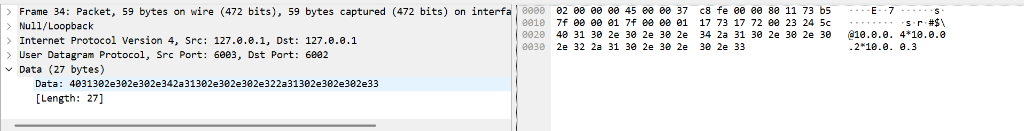
\includegraphics[width=\textwidth]{docs/img/hello_frame34.png}
\caption{Mensagem \textbf{HELLO} (Frame 34): IPv4 \texttt{127.0.0.1 -> 127.0.0.1}, UDP \texttt{6003 -> 6002}, conteúdo \texttt{@10.0.0.4*10.0.0.2*10.0.0.3} (27 bytes).}
\label{fig:hello}
\end{figure}

\begin{figure}[H]
\centering
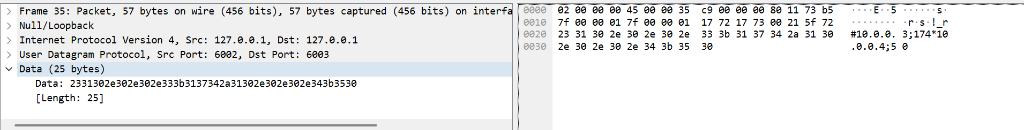
\includegraphics[width=\textwidth]{docs/img/lsa_frame35.png}
\caption{Mensagem \textbf{LSA} (Frame 35): IPv4 \texttt{127.0.0.1 -> 127.0.0.1}, UDP \texttt{6002 -> 6003}, conteúdo \texttt{\#10.0.0.3;174*10.0.0.4;50} (25 bytes).}
\label{fig:lsa}
\end{figure}

\begin{figure}[H]
\centering
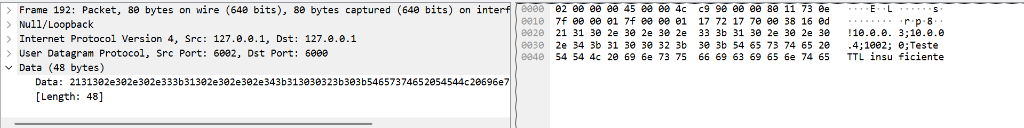
\includegraphics[width=\textwidth]{docs/img/data_frame192.png}
\caption{Mensagem \textbf{DATA} (Frame 192): IPv4 \texttt{127.0.0.1 -> 127.0.0.1}, UDP \texttt{6002 -> 6000}, conteúdo \texttt{!10.0.0.3;10.0.0.4;1002;0;Teste TTL insuficiente} (48 bytes).}
\label{fig:data}
\end{figure}

\end{document}

